\documentclass[11pt]{article}
\usepackage{amsbsy,amsmath,amsthm,amssymb,times,graphicx,enumerate,subfig,color,bbm,float}
\usepackage[latin9]{inputenc}
\usepackage{authblk}
\usepackage[round]{natbib}
\usepackage[text={16cm,24cm}]{geometry}
\usepackage{hyperref}
\setlength{\parskip}{0cm}
\setlength{\parindent}{1em}

\usepackage[compact]{titlesec}
\titlespacing{\section}{0pt}{2ex}{1ex}
\titlespacing{\subsection}{0pt}{1ex}{0ex}
\titlespacing{\subsubsection}{0pt}{0.5ex}{0ex}
%\linespread{0.9}

\renewcommand{\baselinestretch}{2.9}
%\usepackage{subcaption}
\newcommand{\comments}[1]{}
%\newcommand{\pcite}[1]{\citeauthor{#1}'s \citeyearpar{#1}}
\newtheorem{proposition}{Proposition}
\newtheorem{corollary}{Corollary}
\newtheorem{lemma}{Lemma}
\newtheorem{definition}{Definition}
\newtheorem{theorem}{Theorem}
\newtheoremstyle{remboldstyle}
 {}{}{\normalfont}{}{\bfseries}{.}{.5em}{{\thmname{#1 }}{\thmnumber{#2}}{\thmnote{ (#3)}}}
\theoremstyle{remboldstyle}
\newtheorem{remark}{Remark}

%\theoremstyle{remark}
%\newtheorem{remark}{Remark}
%\newtheorem{remark}{\textnormal{\textbf{Remark}}}
\newtheorem{example}{Example}
\setlength{\oddsidemargin}{0.25truein}
\setlength{\evensidemargin}{0.25truein}
\setlength{\textwidth}{6truein}
\setlength{\topmargin}{0.25truein}
\setlength{\textheight}{8.5truein} \setlength{\headsep}{0.0truein}
\setlength{\headheight}{0.0truein} \setlength{\topskip}{10.0pt}

\renewcommand{\baselinestretch}{1.55}
\newcommand{\X}{{\mathsf{X}}}
\newcommand{\Y}{{\mathsf{Y}}}
\newcommand{\cas}{\stackrel{\text{a.s.}}{\longrightarrow}}
\newcommand{\cd}{\stackrel{\text{d}}{\longrightarrow}}
\newcommand{\xn}{\{X_n\}_{n\ge 0}}
\newcommand{\p}{{\boldsymbol{p}}}
\newcommand{\bt}{{\boldsymbol{\theta}}}
\newcommand{\bth}{{\boldsymbol{\theta_1}}}
\newcommand{\bthe}{{\boldsymbol{\theta_2}}}

\newcommand{\x}{{\boldsymbol{x}}}
\newcommand{\y}{{\boldsymbol{y}}}
\newcommand{\oy}{{\boldsymbol{y}_{1}}}
\newcommand{\ty}{{\boldsymbol{y}_{2}}}
\newcommand{\de}{{\boldsymbol{\delta}}}
\newcommand{\ode}{{\boldsymbol{\delta}_{1}}}
\newcommand{\tde}{{\boldsymbol{\delta}_{2}}}
\newcommand{\z}{{\boldsymbol{z}}}

\def\baro{\vskip  .2truecm\hfill \hrule height.5pt \vskip  .2truecm}
\def\barba{\vskip -.1truecm\hfill \hrule height.5pt \vskip .4truecm}
%%%%%%%%%%%%%%%%%%%%%%%%%%%%%%%%%%%%%%%%%%%%
\title{Analysis of Bivariate Survival Data based on copulas with log Generalized Extreme Value marginals}
\author[*]{Dooti Roy}
\author[**]{ Vivekananda Roy}
\author[*]{Dipak Kumar Dey}
\affil[*]{University of Connecticut, Storrs, CT, USA}
\affil[**]{Iowa State University, Ames, Iowa, USA}

\renewcommand\Authands{ and }
%%%%%%%%%%%%%%%%%%%%%%%%%%%%%%%%%%%%%%%%%%%%
\begin{document}
\providecommand{\keywords}[1]{\textbf{\textit{Keywords: }} #1}
%\title{Analysis of Bivariate Survival Data based on copulas with log Generalized Extreme Value marginals}
%\author{Dooti Roy, Vivekananda Roy and Dipak Dey}
\maketitle
%%%%%%%%%%%%%%%%%%%%%%%%%%%%%%%%%%%%%%%%%%%%
\begin{abstract}
\noindent
This chapter introduces a novel copula based methodology to analyze right censored bivariate survival data using flexible log-GEV marginals. Copulas are quite popular in high-dimensional data modeling as they allow modeling and estimating the parameters of the marginal distributions separately from the dependence parameter of the copula. The Clayton copula structure has been used to represent the dependency between the log survival times for this chapter. We propose an empirical Bayes method for estimating the dependency parameter which is more efficient than the other existing Bayesian methodologies. 
\end{abstract}
\keywords{Bivariate survival, Clayton copula, DRS, Empirical Bayes, GEV, Importance Sampling, Metropolis Hastings}
%%%%%%%%%%%%%%%%%%%%%%%%%%%%%%%%%%%%%%%%%%%%
\section{Introduction}
\label{sec:intr}
\noindent
During the last two decades, there have been a growing interest in modeling paired data or bivariate survival data which arises primarily from the field of medicine. For example, it has been medically observed that incidence of one disease often increases the risk of another in a patient affected by Human Immunodeficiency Virus. Diabetic retinopathy is the leading cause of blindness in United States. It has been observed that once one eye gets affected, the chances of the other eye contracting the disease increases many fold. \cite{clayton:1978} and \cite{oakes:1982} were the first to develop a fully parametric approach to model bivariate survival data. In \cite{huster:brookmeyer:self:1989}, the authors extended the fully parametric approach to include censored bivariate paired data with covariates. Since then, between year 1985 to year 1999, several methods using both parametric and semiparametric modeling techniques have been introduced and developed by authors such as: \cite{nelson:1986}, \cite{oakes:1986}, \cite{shih:louis:1995}, \cite{genest:1993} and \cite{wang:wells:2000} among others. Employing copula to model dependency between marginal survival data have been particularly popular since the univariate marginals do not depend on the choice of the dependency structure and can be consequently estimated separately from the dependency parameters.\\
Bayesian methods to model bivariate survival data started developing since early 20's. In \cite{sahu:dey:2000}, the authors used a Bayesian frailty model to model bivariate survival data with covariates. \cite{chen:ibra:sinh:2002} introduced a Bayesian model for right censored bivariate survival data with cure fraction. Another interesting work is by \cite{shem:youn:2000}, where the authors develop a Bayesian joint survival model for life insurance data. In \cite{romeo:tanaka:2006}, the authors used a copula based Bayesian framework to model bivariate survival data. Since choosing an appropriate prior for the dependency parameter of any copula is not intuitive, the authors put a $\beta$-prior on the Kendall's $\tau$ instead. Although these methods are fairly attractive since they are mostly identifiable and produces smooth survival functions, they are not computationally time efficient.
Running MCMC algorithm can be expensive especially when for each individual value of selected $\tau$, MCMC chains for the univariate marginal parameters have to be run. In this chapter, we propose a novel empirical Bayes method of estimating the dependency parameter. Unlike previous works, our method requires only two runs of MCMC chain for the marginal parameters. Our goal is to develop a Bayesian framework for inference and estimation of the marginals and the dependence parameter following the approach outlined in \cite{doss:2010} and \cite{roy:2014} using Clayton copula structure and the flexible Generalized Extreme Value (GEV) distribution to model the marginal distributions. The chapter is organized as follows: Section \ref{sec:intr} provides a brief introduction to the problem and current methods are outlined including their roadblocks and restrictions. In section \ref{sec:cop}, the concept of copula, their properties and different types of copulas have been discussed. In section \ref{sec:marg}, the model settings are described. Our proposed method is outlined in details in section \ref{sec:method}. Section \ref{sec:sim} provides background and results of simulation studies. A real data analysis is provided in the section \ref{sec:drs}. The chapter concludes with future work directions and limitations.
%%%%%%%%%%%%%%%%%%%%%%%%%%%%%%%%%%%%%%%%%%%%
\section{A Brief Overview of Copula}
\label{sec:cop}
\noindent
Copula ``couples" a joint cumulative density function to its marginal distributions and hence the name. Essentially a copula is a bivariate distribution with uniform marginals. The Sklar's theorem (\cite{nelson:1999}, pg:41) defines a copula structure in the following way:\\
Given a $m$-dimensional joint cdf $F$ with marginal cdfs $F_1, F_2, \dots, F_m$, there exists an $m$-copula $C$ such that,
\begin{equation}
  \label{eq:skla}
  F(x_1, x_2, \dots, x_m) = C(F_1(x_1), F_2(x_2), \dots, F_m(x_m))
\end{equation}
for all $(x_1, x_2, \dots, x_m) \in \mathbb{R}^m$. If the marginal distributions are continuous, then $C$ is unique, otherwise $C$ is uniquely determined on Range $F_1 \times \dots \times$ Range $F_m$. Conversely, if $C$ is an $m$-copula and $F_1, F_2, \dots, F_m$ are cdfs, then $F$ defined by \eqref{eq:skla} is an $m$ -dimensional cdf with marginal cdfs $F_1, F_2, \dots, F_m$.\\
Nelson in his book ``Introduction to Copulas (1999)" defined the properties of a $m$-dimensional copula on page 40:
\begin{enumerate}
\item For every $u =(u_1, u_2, \dots, u_m) \in [0, 1]^m$, $C(u) = 0$ if at least
one element $u_i =0$.
\item If all coordinates of $u$ are 1, except $u_i$, then $C(u) = u_i$.
\item For every $a = (a_1, a_2, \dots, a_m), b=(b_1, b_2, \dots, b_m)
  \in [0, 1]^m$, such that $a_i \le b_i$ for all $i = 1, 2, \dots, m$,
  \begin{equation}
    \label{eq:copu}
    \Delta_{a_m}^{b_m} \Delta_{a_{m-1}}^{b_{m-1}} \cdots \Delta_{a_1}^{b_1} C(u) \ge 0,
  \end{equation}
where $\Delta_{a_k}^{b_k}$ defines the first order differences as
\[
\Delta_{a_k}^{b_k} C(u) = C(u_1, \dots, u_{k-1}, b_k, u_{k+1},\dots, u_m) -C(u_1, \dots, u_{k-1}, a_k, u_{k+1},\dots, u_m) .
\]
\end{enumerate}
\noindent
The first and third properties are satisfied if $C(u)$ is a distribution function. The second property is satisfied if the marginal distributions of $C$ are uniform. Using copulas to model dependent bivariate data is advantageous due to many reasons. Copula structure being extremely flexible, allows non-linear dependence between the two associated marginal distributions, or to measure dependence for heavy tailed distributions. It can be used under fully parametric, semi parametric or non parametric setting and also allows for faster computations. Several families of copula have been studied in details, for example: Gaussian copulas, Clayton copulas, Frank copula, Gumbel copula etc. Copula's are chosen depending on the tail concentrations. In this chapter, Clayton copula is chosen to develop the framework and model the Diabetes Retinopathy Study data, since the copula has a nice relationship with the Kendall's $\tau$. Further, \cite{romeo:tanaka:2006} have shown that Clayton copula performs reasonably well on the same real data.
%%%%%%%%%%%%%%%%%%%%%%%%%%%%%%%%%%%%%%%%%%%%
\section{Marginal Distributions and Bivariate Survival Model}
\label{sec:marg}
\subsection{Generalized Extreme Value Distribution as Marginal}
\noindent
\cite{roy:roy:dey:2013} introduced modeling univariate right censored survival data with a cure fraction using Generalized Extreme Value (GEV) distribution (See also \cite{roy:dey:2014}). The GEV distribution characterized by three parameters is extremely flexible and also achieves proper posterior distribution with a variety of mild to diffuse priors. Commonly used lifetime distributions such as the Exponential, the Rayleigh and the Weibull are all special cases of the minima Generalized Extreme Value distribution.\\
If we assume a GEV distribution for $\log T$, where T is a marginal survival time, i.e., $\log T \sim GEV (\mu,\sigma,\xi)$, then the corresponding density and survival functions can be defined respectively as:\\
\[
f(t|\xi)=\begin{cases}
\frac{1}{\sigma t}(1+\xi\frac{(\log t - \mu)}{\sigma})_{+}^{\frac{1}{\xi}-1}\exp[-(1+\xi\frac{(\log t - \mu)}{\sigma})_{+}^{\frac{1}{\xi}}] & \mbox{if} \; \xi  \neq 0\\
\frac{1}{\sigma t}\exp(\frac{\log t - \mu}{\sigma})\exp[-\exp(\frac{\log t - \mu}{\sigma})] & 0<t<\infty; \mbox{if}\ \xi=0.
\end{cases}
\]
\[
S(t|\xi)=\begin{cases}
\exp[-(1+\xi\frac{(\log t - \mu)}{\sigma})_{+}^{\frac{1}{\xi}}]  & \mbox{if}\ \xi\neq0\\
\exp[-\exp(\frac{\log t - \mu}{\sigma})] & \mbox{if} \; \xi=0,
\end{cases}
\]
where $\mu\in \mathbb{R},\; \sigma\in \mathbb{R}^+$ and $\xi\in \mathbb{R}$ are the location, scale and shape parameters respectively. The above distribution was called mGEV in \cite{roy:roy:dey:2013}.
%%%%%%%%%%%%%%%%%%%%%%%%%%%%%%%%%%%%%%%%%%%%
\subsection{Bivariate Model}
\noindent
Let $(T_1, T_2)$ denote failure times of two events for each subject or failure times
of members of each group. Marginally we assume that
\begin{equation}
  \label{eq:marg}
\log T_i \sim \mbox{GEV} (\mu_i, \sigma_i, \xi_i)
\end{equation}
for $i= 1,2$. The joint survival function based on a copula $C_{\phi}, \phi \in G$ is given by
\begin{equation}
  \label{eq:survcop}
  S(\log t_1, \log t_2) = C_\phi (S_1(\log t_1), S_2(\log t_2)),
\end{equation}
where $S_1(\log t_1)$, and $S_2(\log t_2)$ are the marginal survival functions obtained from \eqref{eq:marg}. The parameter $\phi$ measures the ``intensity'' of dependence between the individual failure
times. We use the popular bivariate copula from the Clayton family which is given by
\begin{equation}
  \label{eq:clay}
  C_\phi (u_1, u_2) = \mbox{max} \{(u_1^{-\phi} + u_2^{-\phi} - 1)^{-1/\phi}, 0\} .
\end{equation}
In this case $G= (-1, \infty)\setminus \{0\}$. One of the major goals while studying bivariate data is to gauge the direction and extent of the association between the two variables. When linear correlation coefficient is not a valid measure of association due to nonlinearity of the association, Kendall's $\tau$ and Spearman's $\rho$ are two most popular measures of pairwise concordance \cite[][chapter 5]{nelson:1999}. Certain families of copula have very nice relationship with Kendall's $\tau$. For example, in case of Clayton copula family, the Kendall's $\tau$ measure is given by
\[
\tau_\phi = \frac{\phi}{\phi+2} \in (-1,1).
\]
Due to the easy computation and interpretiblity, Clayton copula remains one of the widely used copula families. 
For proof of the above relationship, see \cite{nelson:1999}, pages 162--163.
%%%%%%%%%%%%%%%%%%%%%%%%%%%%%%%%%%%%%%%%%%%%
\subsection{Model Settings}
\noindent
Let $T_{ij}\; (C_{ij})$ be the survival (censoring) time of the $j$th
event for the $i$th subject, $j=1, 2; i=1, 2,\dots, n$. We assume
$(T_{i1}, T_{i2})$ and $(C_{i1}, C_{i2})$ are independent for
$i=1, 2,\dots, n$. We also assume that $(T_{i1}, T_{i2})$, are iid
with common pdf $f(t_1, t_2)$ and survival time $S(t_1, t_2)$, $i=1, 2,\dots, n$.
The observed data is $(\oy, \ty, \ode, \tde)$, where
$\oy=(y_{11}, y_{21},\dots,y_{n1}), \ty=(y_{12}, y_{22},\dots,y_{n2}),
\ode=(\delta_{11}, \delta_{21},\dots,\delta_{n1})$, and
$\tde=(\delta_{12}, \delta_{22},\dots, \delta_{n2})$, with $y_{ij}
= \log(min (T_{ij}, C_{ij}))$ and $\delta_{ij}= I(y_{ij} = \log T_{ij})$ for
$j=1, 2; i=1, 2,\dots, n$. Let $\y =(\oy, \ty)$ and $\de =(\ode,
\tde)$.  Let $(S_1, S_2)$ and $(f_1, f_2)$ be the marginal survival
and density functions of GEV distribution as given in Section
\ref{sec:marg}.  Let $\mathbf{\bth}$ and $\mathbf{\bthe}$
be the parameters associated with each of the marginal distribution.
So, $\bt_i = (\mu_i, \sigma_i, \xi_i)$, $i = 1,2$. where $\mu,
\sigma$, and $\xi$ are location, scale and shape parameters respectively of the
marginal GEV distributions. \\ Then the complete data likelihood function (joint distribution) of the parameters $(\mathbf{\bth, \bthe}, \phi)$ can be written as (see also \cite{chen:2012}):
\begin{eqnarray}
  \label{eq:lik}
  L(\bth, \bthe, \phi | \y, \de) &=& \prod_{i=1}^n (f(y_{i1}, y_{i2}))^{\delta_{i1} \delta_{i2}}
\Big(\frac{\partial S(y_{i1}, y_{i2})}{\partial y_{i1}}\Big)^{\delta_{i1} (1- \delta_{i2})}
\Big(\frac{\partial S(y_{i1}, y_{i2})}{\partial y_{i2}}\Big)^{(1- \delta_{i1}) \delta_{i2}}
\nonumber\\
&& (S(y_{i1}, y_{i2}))^{(1-\delta_{i1}) (1-\delta_{i2})} \nonumber\\
&=& \prod_{i=1}^n (c_\phi(S_{1 \bth} (y_{i1}), S_{2 \bthe}(y_{i2})) f_{1 \bth}(y_{i1}), f_{2 \bthe}(y_{i2}))^{\delta_{i1} \delta_{i2}}\nonumber\\
&&\Big(-\frac{\partial C_\phi(S_{1 \bth} (y_{i1}), S_{2 \bthe}(y_{i2}))}{\partial S_{1 \bth} (y_{i1})}(-f_{1 \bth}(y_{i1}))\Big)^{\delta_{i1} (1- \delta_{i2})}\nonumber\\
&&
\Big(-\frac{\partial C_\phi(S_{1 \bth} (y_{i1}), S_{2 \bthe}(y_{i2}))}{\partial S_{2 \bthe} (y_{i2})}(-f_{2 \bthe}(y_{i2}))\Big)^{(1-\delta_{i1})\delta_{i2}}\nonumber\\
&&
(C_\phi(S_{1 \bth} (y_{i1}), S_{2 \bthe}(y_{i2})))^{(1-\delta_{i1}) (1-\delta_{i2})} ,
\end{eqnarray}
where $c_{\phi}(.,.)$ is the second derivative of the copula function $C_{\phi}(.,.)$ defined in equation \ref{eq:clay}.
%%%%%%%%%%%%%%%%%%%%%%%%%%%%%%%%%%%%%%%%%%%%
\section{Proposed Methodology}
\label{sec:method}
\noindent
There are mainly two developed approaches to solve the estimation problem. \cite{shih:louis:1995} proposed a two step procedure.  They first assume independence between failure times and estimate the marginals and then estimate the dependency parameter $\phi$ assuming the estimated marginals are fixed. The Bayesian approach simultaneously estimates ($\mathbf{\bth}, \mathbf{\bthe}, \phi$) from joint posterior distribution. The issue with the first approach is the unnatural assumption of independence to begin with. In the second case finding appropriate prior of $\phi$  is difficult because of complicated range depending on which copula family is being used. The dependency parameter for Clayton copula, for example, has the range $ (-1, \infty)\setminus \{0\}$. \\
We start by putting appropriate priors on $\mathbf{\bth}$ and $\mathbf{\bthe}$. Let $\pi(\mathbf{\bth})$ and $\pi(\mathbf{\bthe})$ be the priors on $\mathbf{\bth}$ and $\mathbf{\bthe}$. Then for fixed $\phi$, the joint posterior density of $\mathbf{\bth}$ and $\mathbf{\bthe}$ is given by,
\begin{equation}
  \label{eq:post}
  \pi_\phi(\mathbf{\bth}, \mathbf{\bthe} | \y, \de) = \frac{L(\mathbf{\bth}, \mathbf{\bthe}, \phi| \y, \de) \pi(\mathbf{\bth})
\pi(\mathbf{\bthe})}{m_{\phi}(\y, \de)}, \;\;(\mathbf{\bth}, \mathbf{\bthe}) \in \Theta
\end{equation}
where $m_{\phi}(\y, \de)$ is the normalizing constant given by
\[
m_{\phi}(\y, \de) = \int_{\Theta} L(\mathbf{\bth}, \mathbf{\bthe}, \phi| \y, \de) \pi(\mathbf{\bth})\pi(\mathbf{\bthe}) d\mathbf{\bth} d\mathbf{\bthe}.
\]
Following \cite{roy:2014}, we select that value of $\phi \in G$ which maximizes the marginal likelihood of the data $m_{\phi}(\y, \de)$. Note that $m_{\phi}(\y, \de)$ is not available in closed form and needs to be estimated. Instead of maximizing $m_{\phi}(\y, \de)$, we choose to maximize $a \times m_{\phi}(\y, \de)$ as it is often easier to estimate. We choose ``$a$" as $1/m_{\phi_1}(\y, \de)$ for a pre fixed value $\phi_1$. Then by ergodic theorem, we have a simple importance sampling consistent estimator of $B_{\phi,\phi_1}:= \frac{m_{\phi}(\y, \de)}{m_{\phi_1}(\y, \de)}$.
\begin{equation}
  \label{eq:simbf}
\frac{1}{N} \sum_{l=1}^N \frac{L(\bth^{(l)}, \bthe^{(l)}, \phi| \y, \de)}{L(\bth^{(l)}, \bthe^{(l)}, \phi_1| \y, \de)} \stackrel{a.s.}{\rightarrow} \int_{\Theta} \frac{L(\bth, \bthe, \phi| \y, \de)}{L(\bth, \bthe, \phi| \y, \de)} \pi_{\phi_1}(\bth, \bthe| \y, \de) d\bth d\bthe =\frac{m_{\phi}(\y, \de)}{m_{\phi_1}(\y, \de)},
\end{equation}
as $N \rightarrow \infty$ where $\{\bth^{(l)}, \bthe^{(l)}\}_{l=1}^{N}$  is a single Harris ergodic Markov chain with stationary density $\pi_{\phi_1}(\bth, \bthe| \y, \de)$. So one $\it{single}$ MCMC sample $\{\bth^{(l)}, \bthe^{(l)}\}_{l=1}^{N}$ from $\pi_{\phi_1}(\bth, \bthe| \y, \de)$ is used to estimate $B_{\phi,\phi_1}$ for all $\phi \in G$. Once the association parameter is estimated, $\mathbf{\bth}$ and $\mathbf{\bthe}$ are estimated using Markov Chain (Gibb's sampler) samples from $\pi_{\hat{\phi}}(\bth, \bthe| \y, \de)$.

\subsection{A two-stage procedure}
\label{subsec:twostage}
\noindent
\cite{roy:2014} mentioned that the above estimate of $B_{\phi,\phi_1}$ although simple is often unstable. To remove this instability introduced due to an arbitrary choice of $\phi_1$, following \cite{doss:2010}, \cite{roy:2014} used generalized importance sampling method. Let $\phi_1, \phi_2, \dots, \phi_m \in G$ be $m$ appropriately chosen skeleton points. See \cite{roy:zhu:2014} for a discussion on how to choose the skeleton points. Let $\{\bth^{(j;l)}, \bthe^{(j;l)}\}_{l=1}^{N_j}$ be a Markov chain with stationary density $\pi_{\phi_j}(\bth, \bthe| \y, \de)$ for $j=1\dots,m$. Define $r_k = m_{\phi_k}(\y, \de)/ m_{\phi_1}(\y, \de) $ for
$k = 2, 3, \dots, m$, with $r_1=1$. Then $B_{\phi, \phi_1}$ is consistently estimated by
\begin{equation}
  \label{eq:bf2}
   \hat{B}_{\phi, \phi_1} = \sum_{j =1}^m \sum_{l =1}^{N_j} \frac{ L(\bth^{(j;l)}, \bthe^{(j;l)}, \phi| \y, \de)}{\sum_{k =1}^m N_k L(\bth^{(j;l)}, \bthe^{(j;l)}, \phi_k| \y, \de)/ \hat{r}_k},
\end{equation}
where $\hat {r}_1 =1$, $\hat{r}_k$, $k = 2, 3, \dots, m$ are consistent estimator of $r_k$'s obtained by the ``reverse logistic regression'' method proposed by \cite{geyer:1994} described in details in the next section.
%%%%%%%%%%%%%%%%%%%%%%%%%%%%%%%%%%%%%%%%%%%%%%%%%
\subsubsection{Estimation of $r_k$}
\label{sec:revlog}
\noindent
Following \cite{geyer:1994}, $\hat{r}_k$ are estimated by maximizing the quasi-likelihood fucntion,
\begin{equation}\label{func1}
l_n(r) = \sum\limits_{j = 1}^m\sum\limits_{l = 1}^{N_j} \log p_j(X_{jl},r),
\end{equation}
where $X_{jl} = (\bth^{(j;l)}, \bthe^{(j;l)})$, $r = (r_1, r_2, \dots, r_m)$, $N_j$ is the number of MCMC samples with stationary density $\pi_{\phi_j}(\bth, \bthe| \y, \de)$ corresponding to the skeletal point $\phi_j$, $j = 1, 2,..., m$ and the function $p_j(.,.)$ is defined below. To avoid identifiability issues, $\hat{r_1}$ is assumed to be 1. The function $p_j(.,.)$ is defined as,
\begin{equation}
p_j(X_{jl}, r) = \frac{L(\bth^{(jl)}, \bthe^{(jl)}, \phi_j| \y, \de)e^{r_j}}{\sum\limits_{k = 1}^m L(\bth^{(jl)}, \bthe^{(jl)}, \phi_k| \y, \de)e^{r_k}},
\end{equation}
where $\phi_k$ is the $k^{th}$ skeletal point and $\theta_i^{(jl)} = (\mu_i^{(jl)}, \sigma_i^{(jl)}, \xi_i^{(jl)})$, for $i = 1, 2$ is the $l^{th}$ MCMC sample of the chain with stationary density $\pi_{\phi_j}(\bth, \bthe| \y, \de)$ corresponding to the skeletal point $\phi_j$, $j = 1, 2,..., m$ and $l = 1,...,N_j$.\\
Hence the two-stage procedure for estimating $B_{\phi, \phi_1}$ and $\hat{\phi}$ are as follows. In the first stage, we run MCMC chains $\{\bth^{(j;l)}, \bthe^{(j;l)}\}_{l=1}^{N_j}$ with invariant density $\pi_{\phi_j}(\bth, \bthe| \y, \de)$, $j = 1, 2, ... , m$. We estimate $r$ using these first stage posterior samples using the reverse logistic method as described in section \ref{sec:revlog}. In the second stage, independent of the first stage samples, we obtain $\it{new}$ samples $\{\bth^{(j;l)}, \bthe^{(j;l)}\}_{l=1}^{N_j}$ from $\pi_{\phi_j}(\bth, \bthe| \y, \de)$, $j = 1, 2, ... , m$ to estimate $B_{\phi, \phi_1}$ using equation (\ref{eq:bf2}). Finally, the estimate $\hat{\phi}$ where $\hat{B}_{\phi, \phi_1}$ attains maximum, can be obtained by an optimization procedure or simply looking at the plot of $\hat{B}_{\phi, \phi_1}$ against $\phi$.
%%%%%%%%%%%%%%%%%%%%%%%%%%%%%%%%%%%%%%%%%%%%%%%%
\section{Simulation Study}
\label{sec:sim}
%%%%%%%%%%%%%%%%%%%%%%%%%%%%%%%%%%%%%%%%%%%%%%%%%
\subsection{Generating data}
\noindent
R package ``Copula" was used to generate samples from bivariate distribution with Uniform (0, 1) marginals. The data has dependency according to previously mentioned Clayton copula structure. Next we used ``Inverse Survival Function" approach to get survival times generated from bivariate distribution with $GEV(0,1, \xi)$ marginals. Let $(u_1, u_2) \sim U(0, 1)$. Let $t$ denote the generated survival time. \\
\textbf{Case I: $\xi \neq 0$}
\begin{align}
\begin{split}
1 - u_i = {} &  S(t_i) \\
          = & \exp[-(1 + \xi \log t_i)_{+}^{\frac{1}{\xi}}]
\end{split}\\
\begin{split}
\Rightarrow t_i = {} & \exp[\frac{- 1 + (-\log(1 - u_i))^{\xi}}{\xi}].
\end{split}
\end{align}
\textbf{Case II: $\xi = 0$}
\begin{align}
\begin{split}
1 - u_i = {} &  S(t_i) \\
          = & \exp(-t_i)
\end{split}\\
\begin{split}
\Rightarrow t_i = {} & - \log(1 - u_i).
\end{split}
\end{align}
%%%%%%%%%%%%%%%%%%%%%%%%%%%%%%%%%%%%%%%%
\begin{table}[H]
\caption{Naive Importance Sampling Results for simulated data}
\centering
\begin{tabular}{c c c c}
\hline
$\phi_{1}$ & $Param$      & Estimate[S.E.] & 95\% HPD\\
\hline
1.00          & $\hat{\phi}$ & 5.2114              & -\\
              & $\xi_1$      & 0.308[0.009]        & (0.293, 0.323)\\   
              & $\xi_2$      & 0.312[0.009]        & (0.299, 0.326)\\
              \hline 
2.00          & $\hat{\phi}$ & 5.2116              & -\\
              & $\xi_1$      & 0.308[0.008]        & (0.292,0.322)\\   
              & $\xi_2$      & 0.312[0.006]        & (0.300,0.324)\\
              \hline
4.00          & $\hat{\phi}$ & 5.2116              & -\\
              & $\xi_1$      & 0.307[0.008]        & (0.291,0.321)\\   
              & $\xi_2$      & 0.312[0.007]        & (0.300,0.321)\\
              \hline
6.00          & $\hat{\phi}$ & 5.2115              & -\\
              & $\xi_1$      & 0.308[0.008]        & (0.291,0.322)\\   
              & $\xi_2$      & 0.310[0.009]        & (0.294,0.322)\\
              \hline
8.00         & $\hat{\phi}$ & 5.2117              & -\\
              & $\xi_1$      & 0.308[0.008]        & (0.294,0.322)\\   
              & $\xi_2$      & 0.310[0.008]        & (0.295,0.326)\\
              \hline             
\end{tabular}
\label{tab1}
\end{table}
\noindent
A random sample of 1000 observations were generated following the above method. We selected true $\xi_1 = \xi_2 = 0.3$ and true $\phi = 5$. The choice of $\xi$ were made keeping in mind that in practical scenarios $\xi$ rarely exceeds $[-0.5, 0.5]$ (See \cite{castillo:1997} and \cite{smith:1985}).  Censoring percentages in both $t_1$ and $t_2$ were taken to be about 12\%. 3000 MCMC samples were generated and the first 1000 were discarded as burnin. A uniform prior of (-0.7, 0.7) was considered for $\xi$.  Several initial values of $\phi_1$ were tried. The result of the simulation is displayed in Table \ref{tab1}. Note that due to emirical nature of the estimator, $\hat{\phi}$ has no standard error.
%%%%%%%%%%%%%%%%%%%%%%%%%%%%%%%%%%%%%%%%%%%%
\subsection{Estimation of Parameters}
\begin{table}[H]
\caption{Estimation results for Generalized Importance Sampling}
\centering
\begin{tabular}{c c c }
\hline
$Param$      & Estimate[S.E.] & 95\% HPD\\
\hline
$\hat{\phi}$ &  5.212         & -\\
$\hat{\tau}$ &  0.723         & -\\
$\xi_1$      & 0.308[0.008]        & (0.290, 0.321)\\   
$\xi_2$      & 0.311[0.008]        & (0.298, 0.326)\\
  \hline           
\end{tabular}
\label{tab2}
\end{table}
\noindent
In order to use our multi chain importance sampling method, four skeletal points (2, 4, 6, 8) were selected. We simulated 1000 data points following the method described in section \ref{sec:sim}. The true value of $\phi$ was 5 and $\xi_1 = \xi_2 = 0.3$. For each of the four $\phi$, 3000 MCMC samples were generated. Using the MCMC samples, following \cite{geyer:1994}, first $r_k$, $k = 2, 3, 4$ were estimated (we assume $r_1 = 1$ due to model identifiability issues) and then using them in the second stage, estimate of $\phi$ was obtained. Finally fixing $\phi$ as $\hat{\phi}$, $\xi_1$ and $\xi_2$ were estimated. Table \ref{tab2} provides the details.
%%%%%%%%%%%%%%%%%%%%%%%%%%%%%%%%%%%%%%%%%%%%%%%%%%
\subsection{Note on Monte Carlo Simulation}
\label{sec:note1}
\noindent
Since the extreme value distributions have inter dependent parameters, i.e., the criterion: $1 + \xi \frac{\log t - \mu}{\sigma} > 0$ must always hold, when performing Monte Carlo simulations, there is a need to specify bounds for each parameter contained in the likelihood function. When conducting a real data analysis we assume that both the marginal GEV's have three unknown parameters:$\mu, \sigma$ and $\xi$ in order to allow the data to have maximum flexibility. Also more often than not there is one or more associated covariates. Let us assume that there is one covariate Z for simplicity. We introduce the covariate through $\mu$ parameter as $\mu = \beta_0 + \beta_1Z$. So overall we will have 8 parameters in the likelihood function: $\sigma_1, \xi_1$, $\sigma_2, \xi_2$, $\beta_{01}$ (intercept for log of survival time $y_1$), $\beta_{11}$ (slope for log of survival time $y_1$), $\beta_{02}$ (intercept for log of survival time $y_2$), $\beta_{12}$ (slope for log of survival time $y_2)$.\\
We define the bounds for each of the parameters in the following way:\\
For $\xi$, define $\nu_i = \log y_i - \mu_i, \; i = 1,.., n$. We assume $n$ is the sample size and the standard assumption that $\sigma > 0$ also holds. The parameters $\xi_1$ and $\xi_2$ will have similar bounds. Then,
\[
max(-1, max_{1 \le i \le n}[-\frac{\sigma}{\nu_i}\mathbbm{1}_{\nu_i > 0}]) < \xi < min(1, min_{1 \le i \le n}[-\frac{\sigma}{\nu_i}\mathbbm{1}_{\nu_i < 0}]).
\]
For $\sigma$, define $\zeta_i = \xi (\log y_i - \mu_i), \; i = 1,..., n$. As before, parameters $\sigma_1$ and $\sigma_2$ will have similar bounds. Then,
\[
\sigma > max( 0, max_{1 \le i \le n}(-\zeta_i)).
\]
For the intercept $\beta_0$, we define $A_i = \log y_i + \frac{\sigma}{\xi} - \beta_1 Z_i$. For $\xi > 0$, $\beta_0 \in (-\infty, min A_i)$. For $\xi < 0$, $\beta_0 \in (max A_i, \infty)$.\\
For the slope $\beta_1$, define $B_i = \frac{\log y_i + \frac{\sigma}{\xi} - \beta_0 }{Z_i}$. For $\xi > 0$, $\beta_1 \in (-\infty, min B_i)$. For $\xi < 0$, $\beta_1 \in (max B_i, \infty)$. Note that these bounds hold for postive $Z_i, \; i = 1,...,n$. Further adjustments are needed in case the covariate can take negative values. 
%%%%%%%%%%%%%%%%%%%%%%%%%%%%%%%%%%%%%%%%%%%%%%%%%%%%%
%%%%%%%%%%%%%%%%%%%%%%%%%%%%%%%%%%%%%%%%%%%%%%%%%%%%%
\subsection{Note on Implementation of the Algorithm}
\noindent
In practice, often log likelihood function is used instead of likelihood for scaling issues and also to obtain a simplified form of the full data likelihood. While estimating $r_k$ or $B_{\phi, \phi_1}$ function in the estimation procedure, using likelihood can be a deterrent due to the large magnitude of the evaluated likelihood. One way around this problem is to deal with log likelihood and consider maximizing:
\begin{equation}
l_n(r) = \sum\limits_{j = 1}^m\sum\limits_{l = 1}^{N_j} \log p_j(X_{jl},r)
\end{equation}
where,
\begin{align}
\begin{split}
p_j(X_{jl},r) = {} & \frac{1}{\frac{\sum\limits_{k=1}^{m} e^{L^{*}(\bth^{(jl)}, \bthe^{(jl)}, \phi_k| \y, \de)}e^{r_k}}  {e^{L^{*}(\bth^{(jl)}, \bthe^{(jl)}, \phi_j| \y, \de)e^{r_j}}}}\\
= & \frac{1}{\sum\limits_{k=1}^{m} \frac{ e^{L^{*}(\bth^{(jl)}, \bthe^{(jl)}, \phi_k| \y, \de)}e^{r_k}}  {e^{L^{*}(\bth^{(jl)}, \bthe^{(jl)}, \phi_j| \y, \de)e^{r_j}}}}\\
= & \bigg[\sum\limits_{k=1}^{m} e^{L^*_k - L^*_j} e^{r_k - r_j}\bigg]^{-1},
\end{split}
\end{align}
where $L^*_k = L^{*}(\bth^{(jl)}, \bthe^{(jl)}, \phi_k| \y, \de) = \log  L(\bth^{(jl)}, \bthe^{(jl)}, \phi_k| \y, \de)$. Depending on the converged MCMC chains, the quantity $L^*_k - L^*_j$ should not be overly large and hence the maximization can be carried out. Similar technique can be applied to estimation of maximization of the function $B_{\phi, \phi_1}$ while implementing the second stage of the proposed procedure in the log likelihood function. 
%%%%%%%%%%%%%%%%%%%%%%%%%%%%%%%%%%%%%%%%%%%%%%
\section{Application to Diabetes Retinopathy Study Data}
\label{sec:drs}
\noindent
We consider the well known Diabetes Retinopathy Study (DRS) data for our analyses. This data was first introduced by \cite{huster:brookmeyer:self:1989} in their seminal paper on modeling bivariate data with covariates. The Diabetes retinopathy is the leading cause of blindness in the Unites States under 60 years accounting for approximately 12\% of all new cases. 
It has been shown that 90\% of patients who have been diabetic for more than a decade will evetually develop retinopathy, or an ocular manifestation of blindness. The Diabetes Retinopathy Study (DRS) data consists of 197 patients wth severe retinopathy affecting the eye. For each patient, the data records a treated eye and a control, untreated eye. Time from detection till blindness is the response variable. One or both eye may be censored. The censoring happens in approximately 79\% of the treated eyes and 49\% of the untreated eyes. Age at the onset of diabetes is considered as a covariate.\\ 
\noindent
\cite{huster:brookmeyer:self:1989} analyzed the data using a frequentist approach with the Clayton copula family and Weibull marginal distributions. \cite{th:gram:2000} considered a random effects frailty model and \cite{sahu:dey:2000} considered exponential and Weibull bivariate distributions with a Bayesian approach. \cite{romeo:tanaka:2006} considered copulas to model the dependency of the data and follow the same two step procedures outlined by \cite{shih:louis:1995}. \\
Let us assume time to blindness for the $j^{th}$ eye of the $i^{th}$ patient, $i = 1,...,197$ is $y_{ij}$. Then $\log y_{ij} \sim GEV(\mu_{ij}, \sigma_j, \xi_j)$, $j = 1,2$. The covariate ``age at the time of diagnosis" ($Z$) is included through $\mu_{ij} = \beta_{0j} + \beta_{1j}Z_i,\; j = 1,2$. For simplicity, independent priors are considered on $\sigma, \xi$ and $\beta$. Since we know from subsection \ref{sec:note1}, that the values of the marginal parameters  $\sigma, \xi$ and $\beta$ are all interdependent, we adjust for the dependency by restricting the proposed parameter space within the Monte Carlo simulations. Also, we take $\sigma^2 \sim IG(a_{\sigma}, b_{\sigma})$ and $\xi \sim U(-a, a)$. We pick $a = 1$, $a_{\sigma} = 0.01, b_{\sigma} = 2$ . We put diffuse priors for $\beta_0$s and $\beta_1$s as N(0, 100). The choices of the hyper parameters are such that the posterior distribution is proper.\\
For the first step, following the method outlined in section \ref{sec:method}, an arbitrary $\phi_1 = 3$ value was chosen. Several initial values of $\phi_1$ were tested, however not much difference was observed in the final estimates of the model parameters except the value of $\phi$. \\
Next, using this $\phi_1$, we use the Gibbs sampler with Metropolis-Hastings steps to get the posterior samples for parameters. For this data set, we have 10,000 MCMC iterations. Convergence was checked using the trace plots, ergodic mean plots and the autocorrelation plots for all the parameters. And we find that 4,000 iterations are adequate as burn-in and every $5^{th}$ sample was chosen after thinning. Using 1,200 posterior samples, we then estimate the final $\phi$ value by maximizing $B_{\phi, \phi_1}$. Final estimates and HPD intervals for all 8 parameters were calculated based on the final estimated $\hat{\phi}$. The following table \ref{tab3} provides us the estimates for the parameters.
\begin{table}[H]
\caption{Naive Importance Sampling Results for DRS data}
\centering
\begin{tabular}{c c c}
\hline
$Param$      & Estimate[S.E.] & 95\% HPD\\
\hline
$\hat{\phi}$ & 1.065              & -\\
$\hat{\tau}$ & 0.347              & -\\
$\sigma_1$      & 1.012[0.153]        & (0.743, 1.323)\\   
$\xi_1$      & 0.144[0.165]        & (-0.181, 0.426)\\
$\sigma_2$ & 1.313[0.236]              & (0.911, 1.766)\\
$\xi_2$      & 0.148[0.172]        & (-0.270, 0.403)\\   
$\beta_{01}$      & 2.644[0.299]        & (2.069, 3.229)\\
$\beta_{11}$ & 0.018 [0.013]             & (-0.003, 0.044)\\
$\beta_{02}$      & 2.650[0.391]        & (1.953, 3.454)\\   
$\beta_{12}$      & 0.010[0.017]        & (-0.022, 0.042)\\
 \hline             
\end{tabular}
\label{tab3}
\end{table}
\noindent
However, as the plot demonstrates the estimates obtained from the naive importance sampling are not stable and the function $B_{\phi, \phi_1}$ achieves it's maximum at different points for differnt initial starting values of $\phi_1$. \\
\begin{figure}[H]
\begin{center}
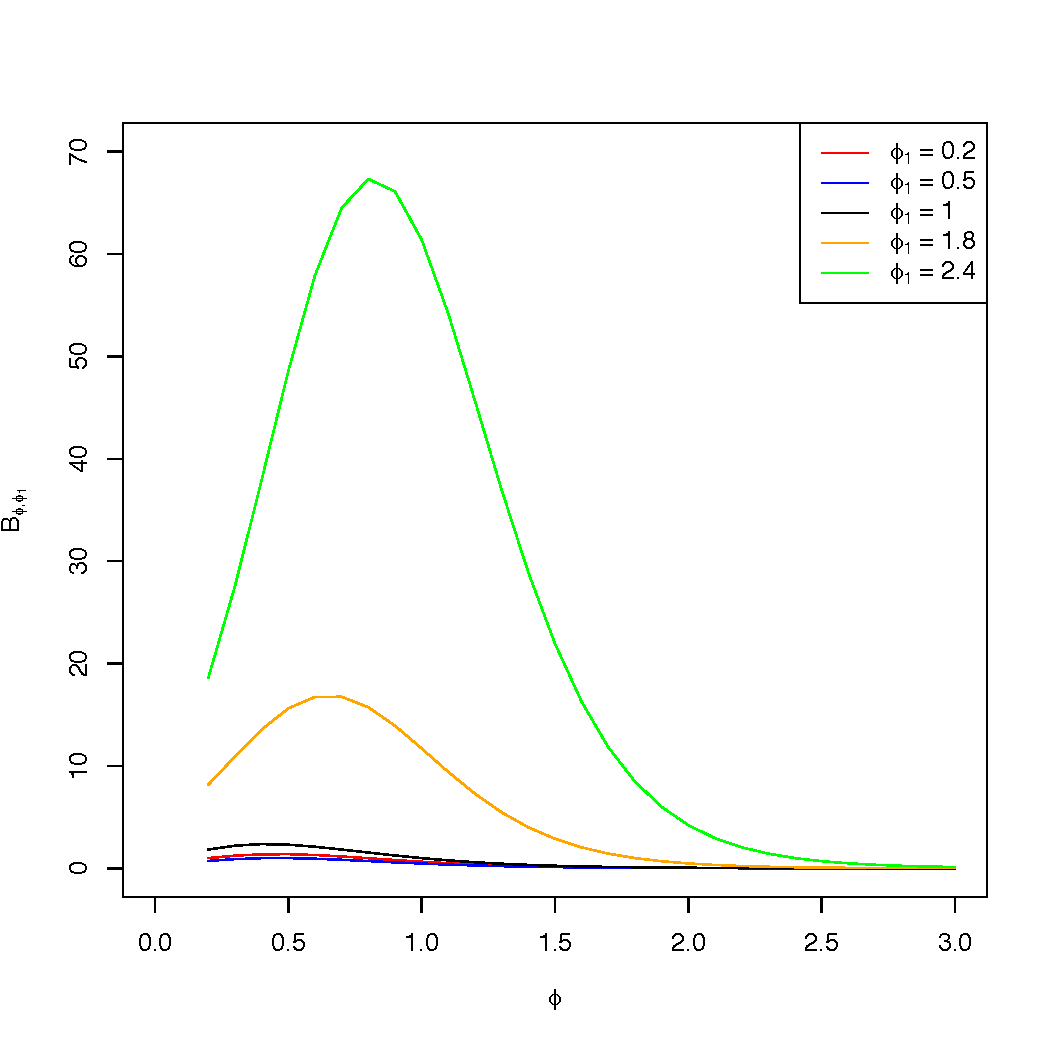
\includegraphics[scale=0.4]{plot1.pdf}
\end{center}
\caption{Plot of $B_{\phi, \phi_1}$ against $\phi$}
\end{figure}
\noindent
In order to obtain stable estimates of the model parameters, following the method outlined in subsection \ref{subsec:twostage}, four skeletal points were chosen as $\phi_1= 0.2$, $\phi_2= 0.5$, $\phi_3= 1$, $\phi_4 = 3$. 10,000 MCMC samples were generated for each skeletal points and 4000 were considered as burn-in after checking for convergence and the chains were thinned every $5^{th}$ sample. The maximum likelihood estimates of the marginal parameters given the value of skeletal point $\phi$ were estimated by maximizing the log likelihood function and were considered as initial starting value for the MCMC simulations. Once all the four MCMC chains were obtained, the function (\ref{func1}) was maximized to obtain estimated $\hat{r}_j$ s. The estimated values of $\hat{r}_j$  were quite robust to the change in initial start values. The following table \ref{tab4} provides the values of $\hat{r}_j$. 
\begin{table}[H]
\caption{Estimated $\hat{r}_j$ for DRS data}
\centering
\begin{tabular}{c c c c c}
\hline
r    & $r_1$  & $r_2$  & $r_3$  & $r_4$ \\
\hline
$\hat{r}$ & 1&  0.679 &  1.445  & 7.867 \\
 \hline             
\end{tabular}
\label{tab4}
\end{table}

\noindent
Using the estimated $\hat{r}_j$ s, $\hat{B}_{\phi, \phi_1}$ was maximized as a function of $\phi$ and the final estimate $\hat{\phi}$ was obtained. Finally, using the estimated $\hat{\phi}$, the marginal parameters were determined using Gibb's sampling algorithm as done before in section \ref{sec:sim}. Table \ref{tab5} provides the final estimates of the model parameters. 
\begin{table}[H]
\caption{Generalized Importance Sampling Results for DRS data}
\centering
\begin{tabular}{c c c}
\hline
$Param$      & Estimate[S.E.] & 95\% HPD\\
\hline
$\hat{\phi}$ & 2.141              & -\\
$\hat{\tau}$ & 0.517              & -\\
$\sigma_1$      & 1.221[0.217]        & (0.814, 1.662)\\   
$\xi_1$      & 0.216[0.162]        & (-0.112, 0.484)\\
$\sigma_2$ & 1.539[0.257]              & (1.053, 2.026)\\
$\xi_2$      & 0.190[0.162]        & (-0.143, 0.446)\\   
$\beta_{01}$      & 2.666[0.326]        & (2.008, 3.243)\\
$\beta_{11}$ & 0.026 [0.014]             & (-0.002, 0.055)\\
$\beta_{02}$      & 2.669[0.4161]        & (1.809, 3.436)\\   
$\beta_{12}$      & 0.019[0.019]        & (-0.015, 0.057)\\
 \hline             
\end{tabular}
\label{tab5}
\end{table}
\noindent
The final estimate $\hat{\phi}$ is quite different from the simple importance sampling estimator obtained in table \ref{tab3}. In \cite{romeo:tanaka:2006}, the authors found the estimated $\hat{\phi}$ to be approximately 1.061. Our estimated $\hat{\phi}$ is higher but in the same direction. The estimated $\hat{\tau}$ is 0.517. It can be thus concluded that the marginal time to blindness for the patients eyes are indeed positively associated. The estimates of slopes of predictor Age are not significant for both the marginals. This finding agrees with Romeo and Tanaka (2006). 
\section{Discussion}
\label{sec:dis}
\noindent
A new bivariate survival model using copula with flexible log Generalized Extreme Value marginals is proposed in this chapter. Since the construction of appropriate priors for the association parameter of the copula may be difficult, an empirical Bayes methodology is developed for making inference on these parameters by maximizing the marginal likelihood function. The proposed method will work on any bivariate data and is not restricted to survival data or to a particular family of copulas. A future direction of work includes extending the proposed methodology for multivariate responses. If the multivariate copula has many association parameters, use of the proposed methodology for estimating these parameters seems challenging. 

\bibliographystyle{plainnat}
\bibliography{copula}
\end{document}